\documentclass[12pt,a4paper]{article}

\usepackage[utf8]{inputenc}
\usepackage[T2A]{fontenc}
\usepackage[ukrainian]{babel}

\usepackage{geometry}
\geometry{left=2cm,right=2cm,top=2cm,bottom=2cm}

\usepackage{graphicx}
\usepackage{array,multirow}
\usepackage{booktabs}
\usepackage{caption}
\renewcommand{\thetable}{\arabic{table}}
\captionsetup[table]{name=Таблиця}
\captionsetup[figure]{name=Рис.}

\usepackage{amsmath}
\usepackage{pdflscape}
\usepackage{xcolor}
\usepackage{hyperref}

\begin{document}

%====================== ТИТУЛКА ======================
\begin{titlepage}
    \begin{center}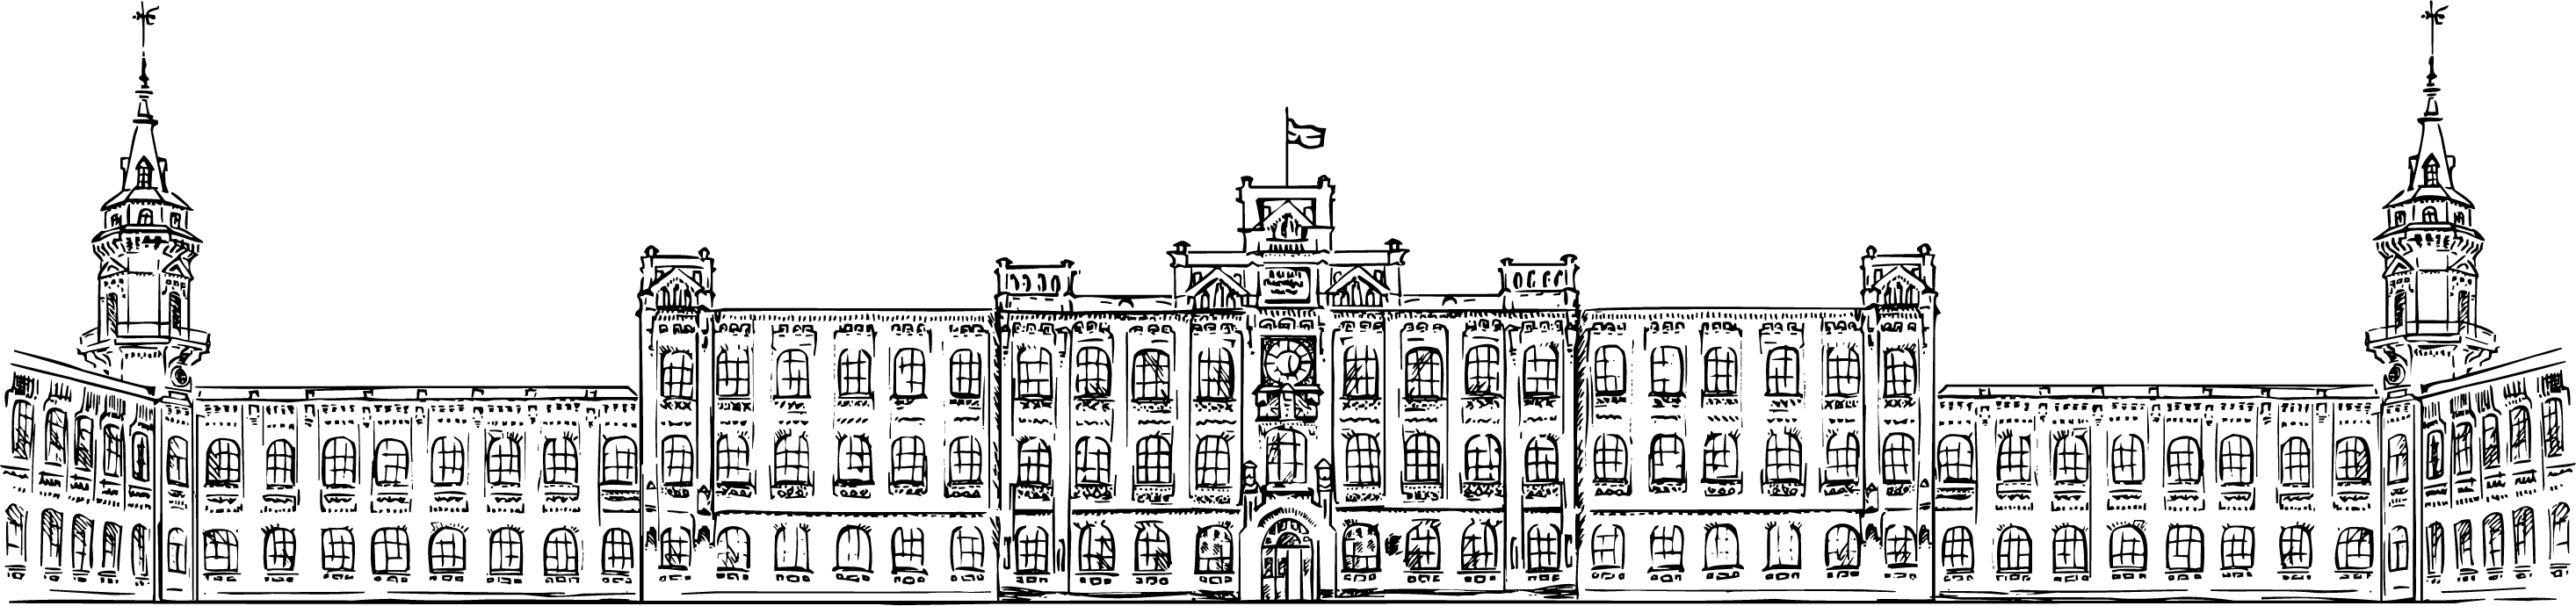
\includegraphics[width=0.7\textwidth]{../../TITLES/letterhead.png}\end{center}

    \begin{center}
        \large Національний технічний університет України\\
        «Київський політехнічний інститут імені Ігоря Сікорського»\\[1em]
        Факультет інформатики та обчислювальної техніки\\
        Кафедра обчислювальної техніки
    \end{center}

    \vfill

    \begin{center}
        \textbf{\LARGE Вступ до філософії}\\[2em]
        \textbf{\Large Доповідь на тему}\\[0.5em]
        «Томас Кун. Структура наукових революцій»
    \end{center}

    \vfill

    \begin{flushright}
        Виконав: студент 2 курсу ФІОТ, гр. ІО-41\\
        \textit{Давидчук А.~М.}\\[1em]
        Перевірив: \textit{Процко С.~А.}
    \end{flushright}

    \vfill

    \begin{center}Київ --- 2025\end{center}
\end{titlepage}

%====================== НАЛАШТУВАННЯ АБЗАЦІВ ======================
\setlength{\parindent}{0pt}

\textbf{\underline{Тема:}} «Т. Кун. Структура наукових революцій».\\[0.6em]
\textbf{\underline{Мета:}} Системно подати зміст концепції наукових революцій, роль парадигм, природу наукового розвитку та їхню сучасну інтерпретацію.

%====================== ВСТУП ======================
\begin{center}\textbf{\large Вступ}\end{center}
\setlength{\parindent}{1.5em}

Книга Томаса Куна «Структура наукових революцій» (1962) стала одним із найвпливовіших творів філософії науки XX століття та змінила уявлення про те, як історично розвивається наукове знання. Кун звернув увагу на те, що наука не є рівномірним поступовим процесом накопичення фактів. Навпаки, її історія складається з періодів стабільності та різких переломів, коли базові уявлення про світ докорінно змінюються. Такі моменти він назвав науковими революціями.

Кун одним із перших запропонував розглядати наукове знання не лише як логічну структуру, але й як соціально-історичну практику, в якій важливу роль відіграють наукові спільноти, їхні норми, методи, освітні традиції та уявлення про допустимі способи пояснення. Завдяки цьому наука постає як складна система, де об’єктивна раціональність поєднується з історичною змінністю.

\vspace{1em}

%====================== ОСНОВНА ЧАСТИНА ======================
\begin{center}\textbf{\large Основні положення праці}\end{center}

\textbf{1. Допарадигмальний етап.}  
До формування зрілої науки існує період, коли різні мислителі пропонують власні теорії та методи, не маючи спільного підходу. Це характерно для ранніх стадій фізики, хімії, медицини. Наука ще не має єдиних стандартів, тому панує конкуренція ідей.

\textbf{2. Парадигма.}  
Центральне поняття Куна — «парадигма». Це не лише певна теорія, а цілий комплекс елементів:
\begin{itemize}
    \item загальні світоглядні принципи;
    \item методи, які вважаються науковими;
    \item стандарти доведення;
    \item моделі розв’язання задач;
    \item підручники, наукові норми та мова.
\end{itemize}
Парадигма визначає, що саме вважається «науковою проблемою» та які розв’язання будуть прийнятні.

\textbf{3. Нормальна наука.}  
Після встановлення парадигми наука входить у стабільний період розвитку. Дослідники займаються «розв’язанням головоломок»: уточнюють параметри, розширюють експериментальні дані, застосовують теорію до нових умов. Важливо, що в цей час парадигма не ставиться під сумнів.

\textbf{4. Аномалії.}  
З часом у межах парадигми накопичуються факти, які не можна пояснити доступними засобами. Спочатку ці аномалії ігнорують або інтерпретують як експериментальні похибки, однак їх зростання створює напруження і підриває довіру до старої парадигми.

\textbf{5. Криза.}  
Коли аномалії стають надто значними, настає криза. Науковці уже не можуть ефективно розв’язувати проблеми старими засобами. Виникають альтернативні теорії та суперечливі пояснення. Наукова спільнота втрачає єдність.

\textbf{6. Наукова революція.}  
Революція відбувається тоді, коли стара парадигма повністю втрачає пояснювальну силу і на її місце приходить нова. Відбувається «парадигмальний зсув»: змінюється весь спосіб наукового мислення. Це не просто уточнення старих теорій — це радикальна перебудова фундаментальних уявлень.

\textbf{7. Нова нормальна наука.}  
Коли спільнота приймає нову парадигму, система стабілізується. Починається новий період нормальної науки, і цикл повторюється.

\vspace{1em}

%====================== КЛЮЧОВІ ІДЕЇ ======================
\begin{center}\textbf{\large Ключові концепції Куна}\end{center}

\textbf{Парадигма як основа наукової раціональності.}  
Певна парадигма задає правила, мову, критерії обґрунтування та навіть бачення того, що є фактом. Тому розвиток науки неможливо звести до суто логічного накопичення знань.

\textbf{Несумірність парадигм.}  
Стара і нова парадигми часто несумірні: вони по-різному бачать світ, формують різні питання, оперують різними поняттями. Представники різних парадигм буквально «говорять різними мовами».

\textbf{Соціальний характер науки.}  
Наука, за Куном, — це діяльність спільноти. Прийняття парадигми часто залежить від консенсусу, традицій, авторитетів та інституційних структур. Це не применшує раціональності науки, але показує її людський, історичний вимір.

\textbf{Проблема об’єктивності.}  
Кун підриває уявлення про абсолютну об’єктивність науки: якщо кожна парадигма задає власні стандарти, то істина стає контекстуальною. Проте Кун не заперечує науковий прогрес — просто показує, що він має революційний, а не лінійний характер.

\vspace{1em}

%====================== ВИСНОВКИ ======================
\begin{center}\textbf{\large Висновки}\end{center}

Праця Томаса Куна стала фундаментальною подією у філософії науки. Вона показала, що наука розвивається не лише через логічні аргументи і накопичення фактів, але й через революційні зміни у світогляді, мовних структурах та соціальних нормах наукової спільноти.  

Концепція парадигмальних зсувів дала змогу по-новому осмислити історичні приклади — від коперніканської революції до становлення квантової механіки.  

Кун зробив науку більш «людською»: він показав, що в основі наукових революцій лежить не тільки логіка, а й психологія, соціологія, культура й історичний контекст. Саме тому його підхід і сьогодні залишається актуальним для осмислення наукового та технологічного розвитку.

\end{document}
